\section{Architectural Views}
This chapter aims to provide information on the general functionalities of the proposed idea 
as well as insights on the implementation methodologies and architectural designs that will be chosen. 
To achieve this representation of the idea, the main resource used will be several UML diagrams.

Firstly, the functionalities of the system will be defined through the scenario views, thereby the logical 
view which will serve as the implementation base of the system will be designed. 
With the two views, several other views such as the process views for some use cases of the system and 
deployment designs will be presented.

All this designing will be based on the Kruchten’s 4+1 views model\cite{ArchitecturalBlueprints4+1}.

\subsection{Scenarios view: Use case analysis}

Use case diagrams are used to represent all the possible scenarios that implement the functionalities specified.

\subsubsection*{Soil moisture use cases}
\begin{figure}[H]
    \centering
    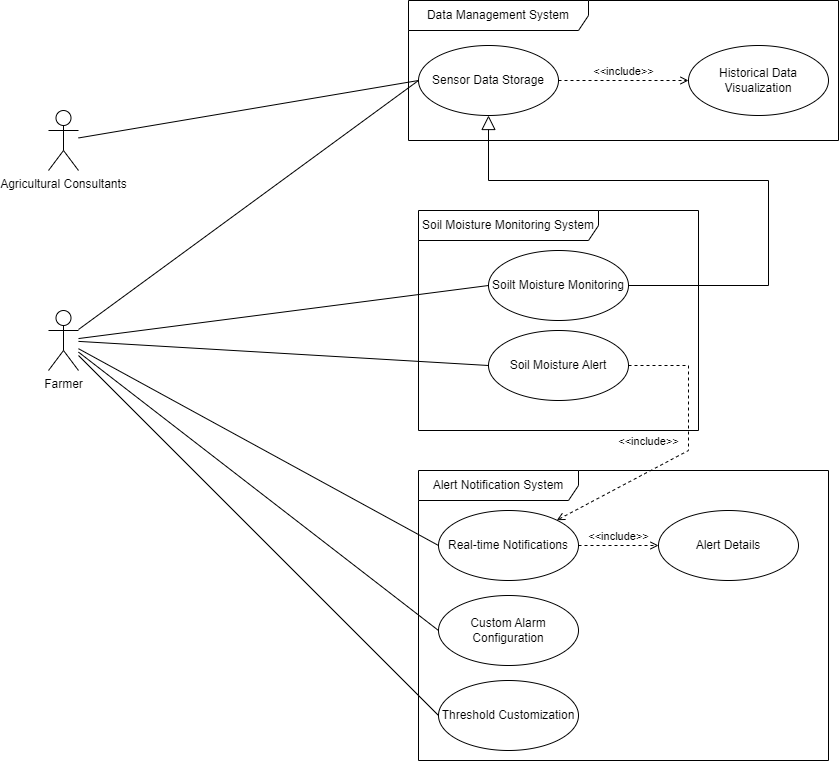
\includegraphics[width=0.8\textwidth]{./images/6/data_soil_alert_uses.png}
    \caption{Soil moisture use cases diagram}
\end{figure}
\todo[inline]{METER LA TABLA DE CASO DE USO}

\subsubsection*{Animal detection system use cases}
\begin{figure}[H]
    \centering
    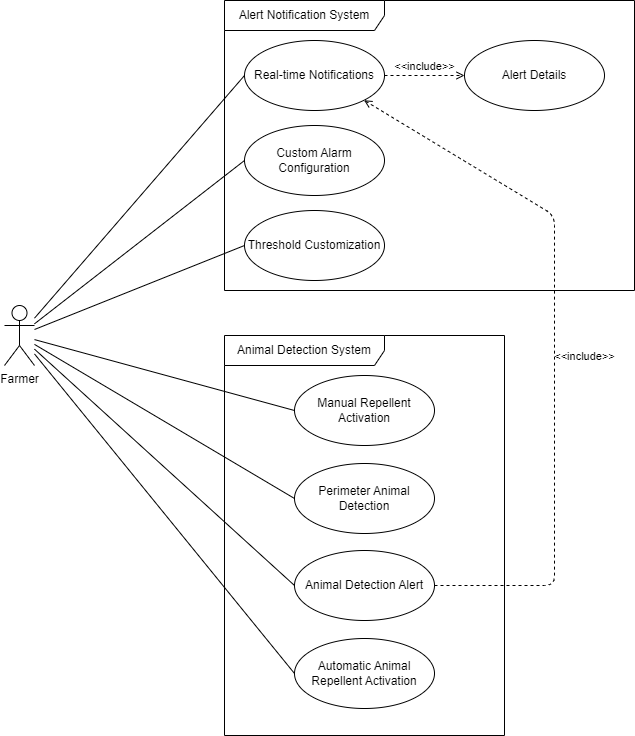
\includegraphics[width=0.8\textwidth]{./images/6/alert_animal_uses.png}
    \caption{Animal detection system use cases diagram}
\end{figure}
\todo[inline]{METER LA TABLA DE CASO DE USO}

\subsubsection*{User management system use cases}
\begin{figure}[H]
    \centering
    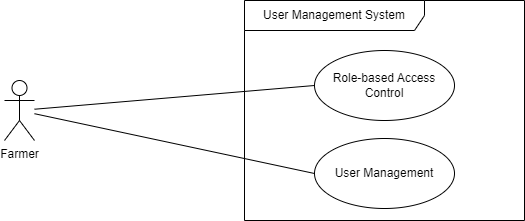
\includegraphics[width=0.8\textwidth]{./images/6/user_management_uses.png}
    \caption{User management system use cases diagram}
\end{figure}
\todo[inline]{METER LA TABLA DE CASO DE USO}

\subsubsection*{Fire detection system use cases}
\begin{figure}[H]
    \centering
    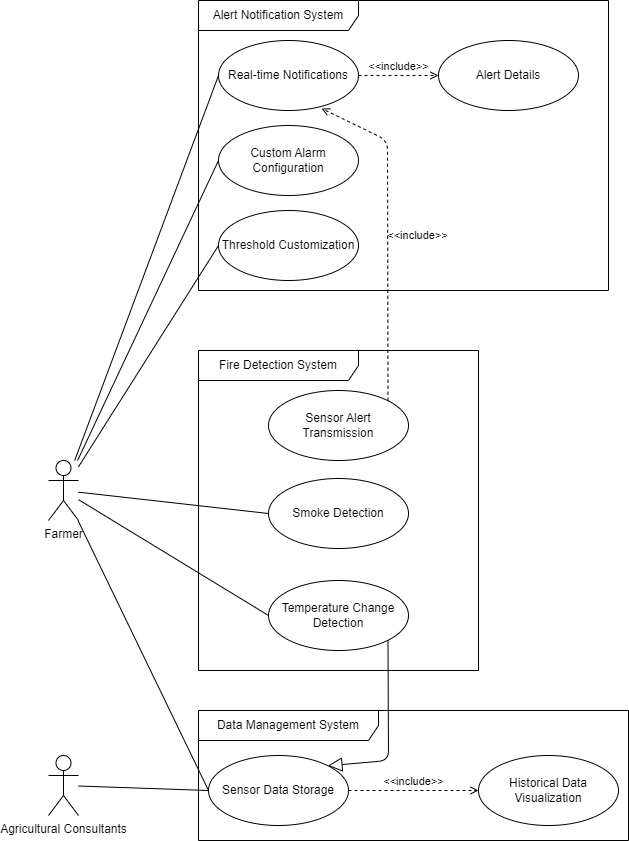
\includegraphics[width=0.8\textwidth]{./images/6/fire_uses.png}
    \caption{Fire detection system use cases diagram}
\end{figure}
\todo[inline]{METER LA TABLA DE CASO DE USO}

\subsubsection*{Energy system use cases}
\begin{figure}[H]
    \centering
    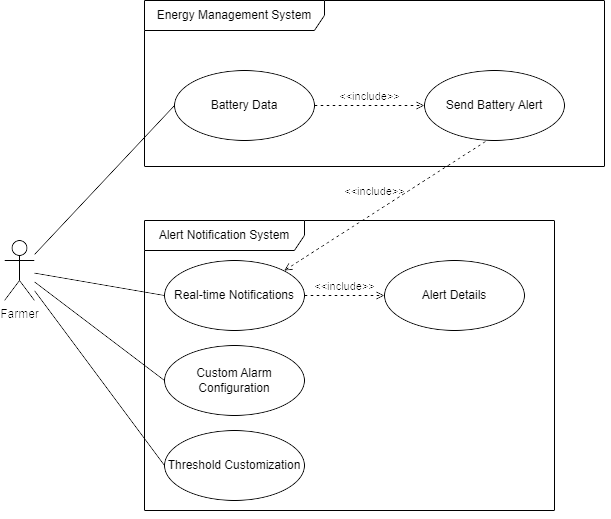
\includegraphics[width=0.8\textwidth]{./images/6/energy.png}
    \caption{Energy system use cases diagram}
\end{figure}
\todo[inline]{METER LA TABLA DE CASO DE USO}

\subsubsection*{Weather monitoring use cases}
\begin{figure}[H]
    \centering
    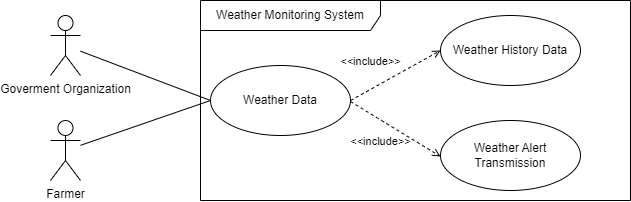
\includegraphics[width=0.8\textwidth]{./images/6/weather_uses.png}
    \caption{Weather monitoring use cases diagram}
\end{figure}
\todo[inline]{METER LA TABLA DE CASO DE USO}